\chapter{Evaluation}
\label{ch:evaluation}
To evaluate RDF-Doctor, firstly, it was tested against standard test cases, including formats of correct and incorrect syntax in files, secondly, to get rid of bias, a random number of errors was generated using Poisson distribution and uniform random number generators for a period of time of 8 hours to simulate a couple of syntax errors, produced by an ontology user, lastly, the performance of RDF-Doctor was measured when both the number of errors and the volumes of ontologies are varied. This chapter discusses all of such experiments in the following text. 
\section{Implementation}
Experiments were run on a Linux
Ubuntu 18.04 machine with a 4th Gen Intel Core i5-
4300U CPU, 3MB Cache, 2.90GHz with 8GB RAM
1333MHz DDR3. RDF-Doctor was implemented using
Java version 9. ANTLR framework version 4.7.1 was used to build the internal parser in RDF-Doctor, as well, as an imported library for compiling and running of it.  

\section{Experiment 1: Validating with RDF Suite Test} In this experiment, RDF-Doctor was validated against RDF Suite Test, specifically Turtle serialization. Next text discusses the objective, shows the procedure, and finally, presents and discusses the result.     
\subsection{Objective}
The evaluation phase starts with \cite{TurtleTests:Online} where Test Suite files of Turtle serialization are found. There are multiple Test Suites for each of RDF serializations, recommend by W3 Consortium\footnote{https://www.w3.org/}. The proficiency of a parser for a certain serialization can be validated with these files found in a corresponding Test Suite. Therefore, the target of this experiment is to measure the proficiency of RDF-Doctor while testing with W3C Turtle Test Suite.

\subsection{Procedure}
Files at \cite{TurtleTests:Online} were prompted to validate a parser that parses a Turtle serialization, hence, it was used to test RDF-Doctor. Metrics of the experiment are both Precision and Recall, donated by equation \ref{eq:1} and \ref{eq:1} sequentially. The former measures the percentage of errors which correctly flagged as syntax errors, while the latter calculates the percentage of actual syntax errors which correctly recognized. Total number of files at \cite{TurtleTests:Online} is 275, divided to parts: files include  correct syntaxes; and files contain incorrect syntaxes, the latter is represented with 65 files, and the remaining are related to the former, as demonstrated by Table \ref{tab:TurtleSuit}. 
 
\begin{table}[]
\centering
\begin{tabular}{|l|l|l|l|}
\hline
\begin{tabular}[c]{@{}l@{}}Error Type Classification \end{tabular} & Detected & \begin{tabular}[c]{@{}l@{}}Not detected\end{tabular} & Total \\ \hline
 Escape Characters              &      0    &    4 &   4  \\ \hline
 Bad Keywords             &      5   &    0 &   5  \\ \hline
 Bad Literals with langTag             &      2   &    0 &   2  \\ \hline
 Bad Local Name-space in IRI             &      2   &    3  &   5  \\ \hline
 Bad Namespace in IRI             &      2   &    0 &   2  \\ \hline
 N3 Extra             &      11   &    1 &   12  \\ \hline
 Bad Namespace in Directives             &      2   &    0 &   2  \\ \hline
 Bad Number as a Literal             &      5   &    0 &   5  \\ \hline
 Bad Directives             &      4   &    0 &   4  \\ \hline
 Bad Strings             &      6   &    1 &   7  \\ \hline
 Bad Structures            &      12   &    0 &   12  \\ \hline
 Bad IRI            &      2   &    3 &   5  \\ \hline
 Total            &      53   &    12 &   65  \\ \hline
\end{tabular}
\caption{\textbf{Evaluation of RDF-Doctor against detection of incorrect syntactic forms in Turtle Test Suite \cite{TurtleTests:Online}.} The test focuses on the files, including  an incorrect Turtle syntax,  ”Detected” in pointed to recognized syntactic forms as incorrect forms with releasing corresponding error messages, but ”Not detected” specifies incorrect syntactic forms which are not recognized and might generate false positives.}
\label{tab:detection}
\end{table}

\subsection{Result and Discussion}

The test drives the result when dealing with either correct or incorrect Turtle syntax. Thus, correct syntaxes should be recognized as correct, similarly in case of incorrect syntaxes plus exception errors should be fired.  However,  the test result in Table \ref{tab:TurtleSuit} shows recognizes mostly of correct syntaxes with 88\%, while the remaining 12\% RDF-Doctor are not recognized and it consider them as errors. In the meanwhile, when dealing with incorrect syntaxes, again, Table \ref{tab:TurtleSuit} provides that 81,5\% of files included incorrect syntaxes are detected and an error message was fired for each one of them, the rest 17,5\% go without being identified as incorrect forms, as well as no errors were fired.



\begin{table}[]
\centering
\begin{tabular}{|l|l|l|l|}
\hline
\begin{tabular}[c]{@{}l@{}}File Content \end{tabular} & Detected  & Not detected & Total \\ \hline
 Correct Syntax              &      185    &      25  & 210 \\ \hline
 Incorrect/Bad Syntax              &      53    &    12  & 65 \\ \hline
 Total            &      238   &       37 & 275  \\ \hline
\end{tabular}
\caption{\textbf{Evaluation summary of RDF-Doctor for both correct and incorrect syntactic forms when validating with Turtle Test Suite \cite{TurtleTests:Online}.} "Detected" for Correct Syntax means that RDF-Doctor is able to recognize them as correct syntactic forms, whereas, for those which are not correctly recognized classified under "Not detected", similarly, "Detected" in Incorrect/Bad Syntax referred to recognized syntactic forms  as incorrect forms with releasing corresponding error messages, but "Not detected" specifies  incorrect syntactic forms  which are not recognized and might generate false positives.}
\label{tab:TurtleSuit}
\end{table}

\begin{figure}[ht]
\begin{center}
		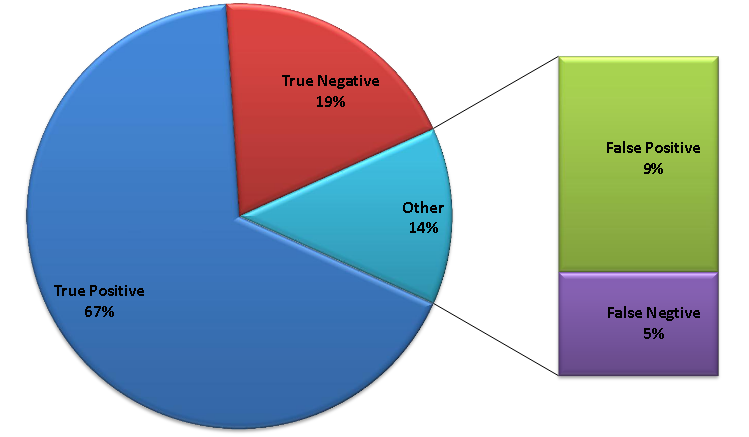
\includegraphics[scale=0.5,angle=0]{images/PieChartExperiment1.png}

		\label{Fig:pieChartExperiment1}
		\caption{\textbf{Result of Experiment 1 to evaluate  RDF-Doctor with Turtle Test Suite \cite{TurtleTests:Online}.} }
\end{center}
\end{figure}

For evaluation, the precision and recall are computed using the equations \ref{eq:1} and \ref{eq:2} respectively.  
\begin{align} 
   Precision=  \frac{t_p}{t_p+f_p}\,;\qquad
\qquad\parbox{4.0cm}{\footnotesize$\begin{aligned} t_p &= \text{ number of true positives}\\[-1.0ex] f_p &= \text{ number of false positives}\end{aligned}$}
   \label{eq:1}
\end{align}
\begin{align}
   Recall =  \frac{t_p}{t_p+f_n} \,;\qquad
\qquad\parbox{4.0cm}{\footnotesize$\begin{aligned} t_p &= \text{ number of true positives}\\[-1.0ex] f_n &= \text{ number of true negatives}\end{aligned}$}
   \label{eq:2}
\end{align}



\section{Experiment 2: Validating with Random Syntax Errors Generation}
\subsection{Objective}
To get rid of the generated bias, this experiment uses both Poisson distribution and uniform random number generation methods. It also assumes a naive user editing an RDF input data, found in an environment similar to the one in Figure \ref{Fig:Motivation} and he is mistakenly generating some  syntax errors. Then, the inserted syntax errors evaluate the quality of RDF-doctor.


\subsection{Procedure}
 In this experiment, a naive user who is working on on RDF input data for 8 hours and each one hour he is making a text change (insert/modify/delete) before submission to RDF-Doctor for parsing is simulated. The average number of making syntax errors per time interval is represented by a parameter $\lambda$. For example, if   $\lambda$ = 5, it means that five syntax errors are occurred per hour.  As an input for a Poisson distribution, 10 syntax errors per instance of time was supplied. Hence, for each instance of time we calculate value of $\lambda$, then the output value drives how many number of syntax errors are entitled for that instance of time. Next, Those syntax errors are arbitrarily selected from the type of errors range [1-61], drawn by rows of Table \ref{tab:syntaxErrorCate}. Beside locations of injected syntax errors were done in a semi-random method, usin  

\subsection{Result and Discussion}



	\begin{figure}[ht]
	\begin{center}
		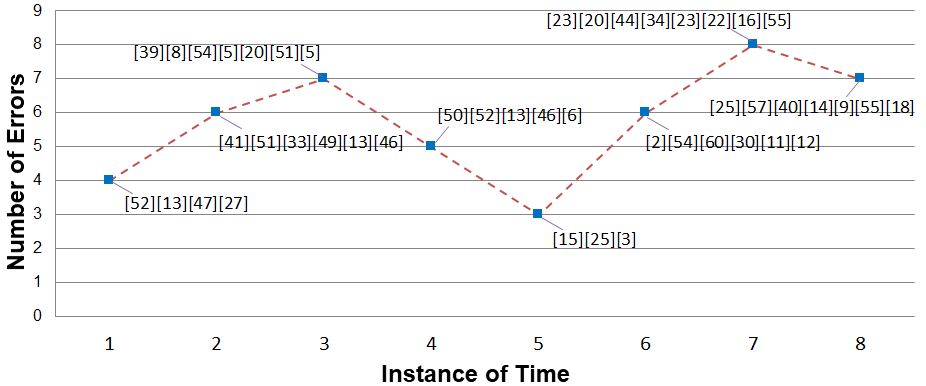
\includegraphics[scale=0.45,angle=0]{images/Experiment02-01.png}
		\setlength\belowcaptionskip{-5mm}
		\caption{\textbf{Random syntax errors distribution.} Number and types of syntax errors between brackets for a user in an interval of 8 instances of time. A Poisson  distribution with $\lambda$ = 5 models an average of 5 syntax errors per instance of time. Each instance of time shows value of$\lambda$, assuming the user can generate [1-10] syntax errors per instance of time. A uniform random number generator computes type of errors from [1-61] syntax errors in Table \ref{tab:syntaxErrorCate}.} 
		\label{Fig:experiment2}
	\end{center}
\end{figure}



	\begin{figure}[ht]
	\begin{center}
		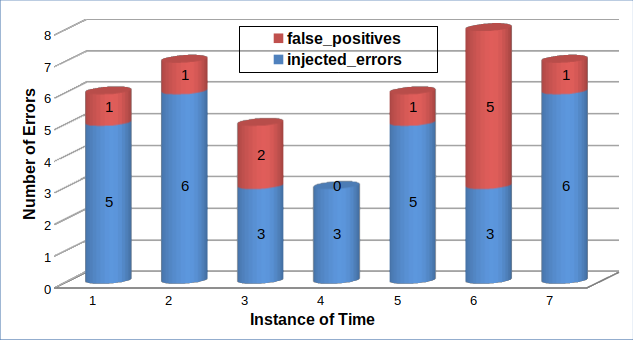
\includegraphics[scale=0.7,angle=0]{images/Experiment02-02.png}
		\setlength\belowcaptionskip{-5mm}
		\caption{\textbf{Result of error detection when syntax errors are randomly generated.}} 
		\label{Fig:Experiment02-02}
	\end{center}
\end{figure}

	\begin{figure}[ht]
	\begin{center}
		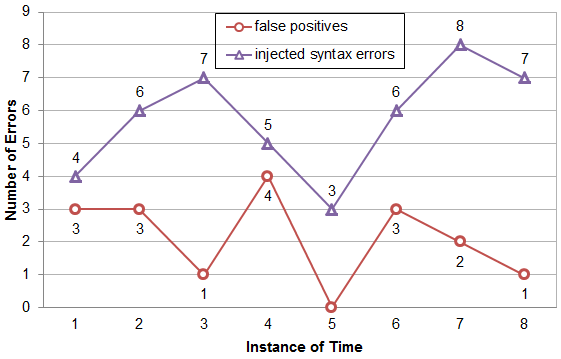
\includegraphics[scale=0.7,angle=0]{images/Experiment02-03.png}
				\setlength\belowcaptionskip{-5mm}
		\caption{\textbf{Result of False Positives in Experiment 2 when syntax errors are randomly generated.}} 
		\label{Fig:Experiment02-03}
				\setlength\belowcaptionskip{-5mm}
		\setlength\abovecaptionskip{0mm}
	\end{center}
\end{figure}

\section{Experiment 3: Impact of Number of Errors and  Volume on Behaviour and  Performance}
\subsection{Objective}

In order to study the behaviour and the performance of RDF-Doctor, this experiment was performed. We are studying the effect of growing of number of syntax errors, as well as, the size of ontologies when it is changed. 


\subsection{Procedure}
Two types of ontologies are used: small; and medium size. For the former, FOAF  (an abbreviation form of friend of a friend) Vocabulary\footnote{http://www.foaf-project.org/} was used, it is a small ontology with volume of about 23.3 Kbyte, including people-related terms. Whilst the latter made use of the ontology  of DBpedia schema\footnote{https://wiki.dbpedia.org/develop/datasets/dbpedia-version-2016-10}, version 2016-10, with volume of about 4.1 Mbyte, including meta-data about all contained datasets of DBpedia. Both datasets were used 3 times and for one time 10, 30, 61 syntax errors were randomly  injected using the same procedure of uniform random generation. Additionally, to evaluate the performance of RDF-Doctor, same 6 of the datasets were parsed for 5 times to get the average of processing time  

 
\subsection{Result and Discussion}
Figure \ref{Fig:Experiment03-01} drives the impact of number of errors and the volume size. When introducing 10 syntax error, 9 out 10 were detected and one was not detected for both FOAF and DBpedia. 25 out 30 injected syntax errors in FOAF and 26 out 30 injected syntax errors in DBpedia were detected, the rest are undetected. Subsequently, 61 syntax errors were inserted 6 and 11 syntax errors go undetected in FOAF, DBpedia, respectively, the remaining are detected with expressive error messages to help users in resolving such errors. 
\begin{figure}[ht]
\begin{center}
		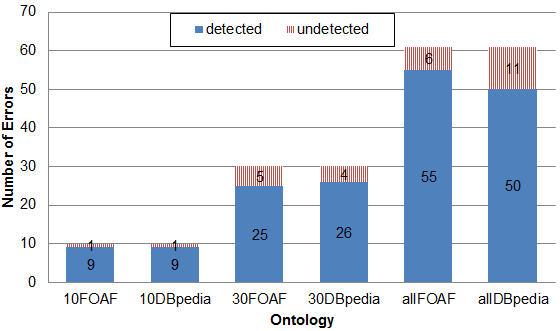
\includegraphics[scale=0.45,angle=0]{images/Experiment03-01.png}
				\setlength\belowcaptionskip{-5mm}

		\caption{\textbf{Result of Experiment 3 to evaluate the impact of number of errors and volume on RDF-Doctor.} FOAF, and DBpedia ontologies were used to evaluate RDF-Doctor, 10foaf, 30foaf, allfoaf are datasets of FOAF ontology, including with 10, 30, 61 random syntax errors, respectively, same is applicable for DBpedia. Detected errors are the errors which were properly identified by RDF-Doctor and the matched error messages were released, while undetected errors are those which not correctly recognized.}
		\label{Fig:Experiment03-01}

\end{center}
\end{figure}


Another essential point is number of false positives were shown in the result, as it is demonstrated  by Figure \ref{Fig:Experiment03-02}. Clearly, it can be seen that the false positives  are incremented while raising of the number of syntax errors, that comes as consequence of increasing number of unrecognized syntax errors, then the parser tries to recover from such errors by adding or removing some tokens which produces more and more false positives.   




\begin{figure}[ht]
\begin{center}
		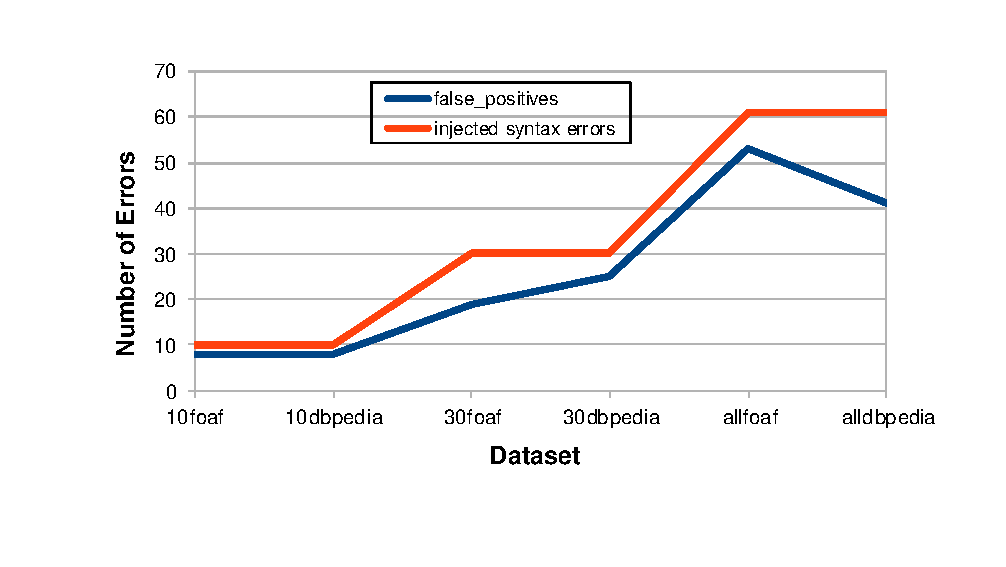
\includegraphics[scale=0.9,angle=0]{images/Experiment03-02.pdf}
		\setlength\belowcaptionskip{-5mm}
		\setlength\abovecaptionskip{-15mm}
		\caption{\textbf{Result of False Positives in Experiment 3.} Undetected errors generate false-positive errors and when the number of errors increase, the false-positives are comparably increased.}
				\label{Fig:Experiment03-02}
\end{center}
\end{figure}

Due to the need to measure the RDF-Doctor performance, Figure \ref{Fig:Experiment03-03} was presented. it summaries the impact of both number of errors and volume on RDF-Doctor performance, where numbers of errors has no influence on the performance, as the processing time similar result in either FOAF or DBpedia while changing number of errors. In the meanwhile, volumes has a high impact on the performance, since  DBpedia  takes about 29000 ms in average to be processed, whereas, FOAF was parsed in about 2000 ms.   

To conclude this experiment, It can be seen that number of error detection is promising, more than 90\% of injected syntax errors were detected, as Figure \ref{Fig:Experiment03-01} talks. Also, number of false positives can be improved if RDF-Doctor recognized those undetected errors by either do more laboratory works to match those patterns or may with the new versions of ANTLR library.  
%talk about the correction of errors #numbers 
\begin{figure}[ht]
\begin{center}
		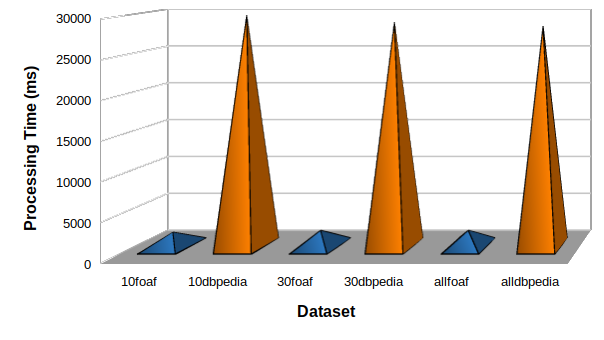
\includegraphics[scale=0.7,angle=0]{images/Experiment03-03.png}
		\setlength\belowcaptionskip{-5mm}
		\setlength\abovecaptionskip{0mm}
		\caption{\textbf{RDF-Doctor performance evaluation when number of errors and volume sizes are varied.} Performance is measured with the processing time in (ms) of FOFA ontology (23.3 Kbyte) and DBpedia ontology (4.1 Mbyte) with 10, 30, and 61 (refereed as all) injected syntax errors.}
				\label{Fig:Experiment03-03}

\end{center}
\end{figure}
